\documentclass[12pt, 
hyperref={colorlinks=true, linkcolor=blue, urlcolor=cyan}]{beamer}
\usetheme{default} 

\setbeamertemplate{navigation symbols}{} %gets rid of navigation symbols
\setbeamertemplate{footline}{} %gets rid of bottom navigation bars
\setbeamertemplate{footline}[page number]{} %use this for page numbers

\setbeamertemplate{itemize items}[circle] %round bullet points
\setlength\parskip{10pt} % white space between paragraphs

\usepackage{wrapfig}
\usepackage{subfig}
\usepackage{setspace}
\usepackage{enumerate}
\usepackage{graphicx}
\usepackage{amsmath}
\usepackage{amsfonts}
\usepackage{amssymb}
\usepackage{amsthm}
\usepackage[UKenglish]{isodate}
\cleanlookdateon

% the preamble
\title{BIOST 311: \\ Regression Methods for the Health Sciences}
\author{Kelsey Grinde and Brian Williamson}
\institute{UW Biostatistics}
\date{Spring 2018}

\begin{document}
% title slide
\begin{frame}
\titlepage\thispagestyle{empty}
\end{frame}

% make it 1.something
\setbeamertemplate{footline}{%
  \raisebox{5pt}{\makebox[\paperwidth]{\makebox[120pt]{\scriptsize Last updated \today}\hfill\makebox[10pt]{\scriptsize 1.\insertframenumber~~}}}}  \newcounter{chap1}{\value{1}}
\setcounter{framenumber}{\value{chap1}}

\begin{frame}
\frametitle{CHAPTER 1: LINEAR REGRESSION}
\end{frame}

\section{Simple Linear Regression}
\begin{frame}
\frametitle{SECTION 1: SIMPLE LINEAR REGRESSION}
\end{frame}

\section{Multiple Linear Regression}
\begin{frame}
\frametitle{SECTION 2: MULTIPLE LINEAR REGRESSION}
By the end of Section 2, you should be able to:

\begin{itemize}
\item Identify potential variables that \textcolor{red}{confound} the association between the predictor of interest and the outcome, and
\item describe \textbf{why} you will adjust for these variables in a regression analysis.
\item Identify potential variables that \textcolor{blue}{modify} the association between the predictor of interest and the outcome, and  
\item describe \textbf{how} you will test for  differential effects.
\item Identify potential variables that help \textcolor{green}{reduce the variability} of our estimates.
\item \textbf{Interpret} parameters in a multiple linear regression model.
\item \textbf{Fit} multiple linear regression models in \texttt{R}, and
\item \textbf{interpret} the output to perform hypothesis tests.
\end{itemize}

\end{frame}

\begin{frame}
\frametitle{Multiple regression: motivation}

So far, we have considered the relationship between the outcome, $Y$, and a \textcolor{green}{single} predictor of interest, $X$.

However, there may be other variables that influence the association between our predictor of interest and the outcome, by:
\begin{itemize}
\item \textcolor{red}{confounding} the association 
\item \textcolor{blue}{modifying} the association
\item providing information that \textcolor{green}{reduces the variability} of our estimates
\end{itemize} 
\end{frame}

\begin{frame}
\frametitle{Multiple regression: motivation}
What do you think the relationship is between $X_1$ and $Y$?

\vspace{-0.3cm}
\centering
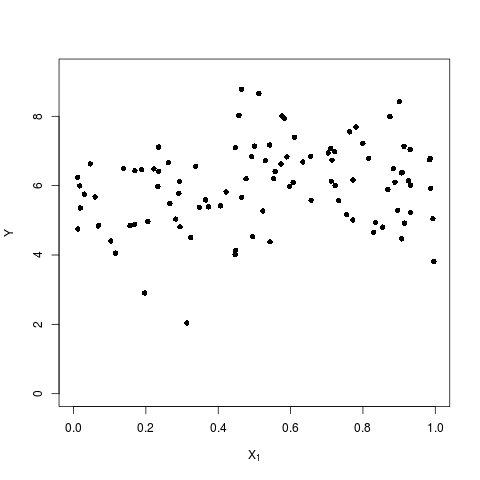
\includegraphics[width = 0.7\textwidth]{plots/confounding_simple.png}
\end{frame}

\begin{frame}
\frametitle{Multiple regression: motivation}
What do you think the relationship is between $X_1$ and $Y$?

\vspace{-0.3cm}

\centering
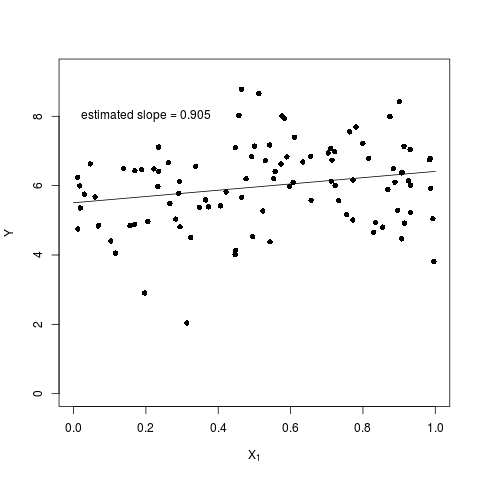
\includegraphics[width = 0.7\textwidth]{plots/confounding_simple_with_line.png}
\end{frame}

\begin{frame}
\frametitle{Multiple regression: motivation}
How about now?

\vspace{-0.3cm}
\centering
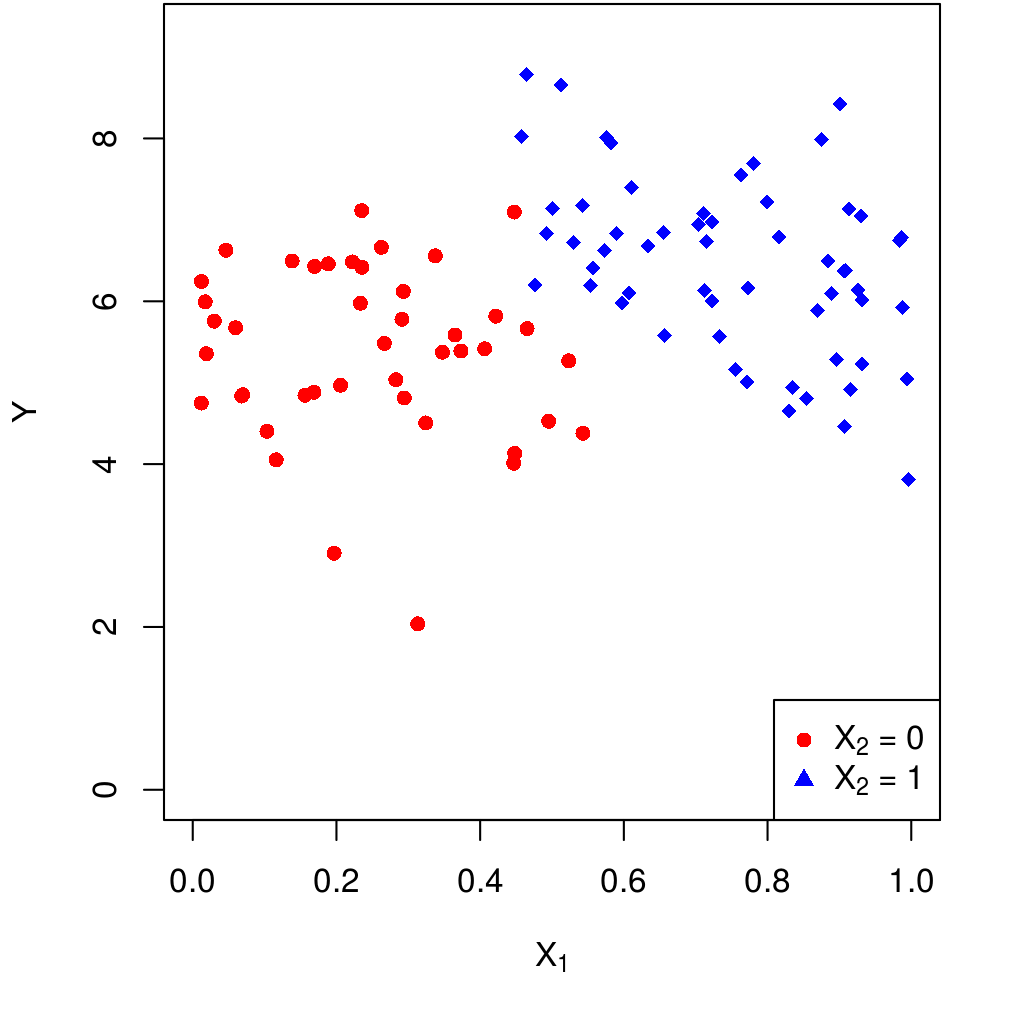
\includegraphics[width = 0.7\textwidth]{plots/confounding_colored.png}
\end{frame}

\begin{frame}
\frametitle{Multiple regression: motivation}
How about now?

\vspace{-0.3cm}
\centering
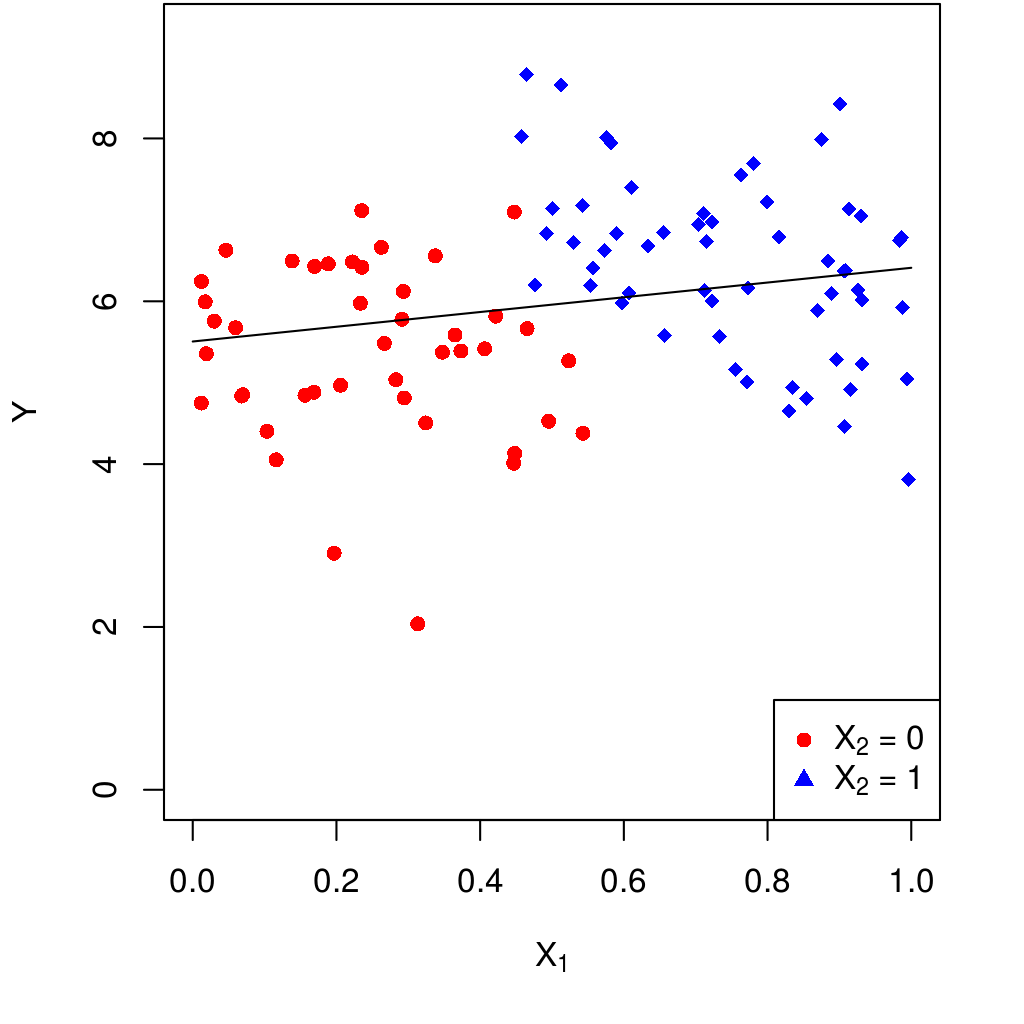
\includegraphics[width = 0.7\textwidth]{plots/confounding_colored_with_simple_line.png}
\end{frame}

\begin{frame}
\frametitle{Multiple regression: motivation}
How about now?

\vspace{-0.3cm}
\centering
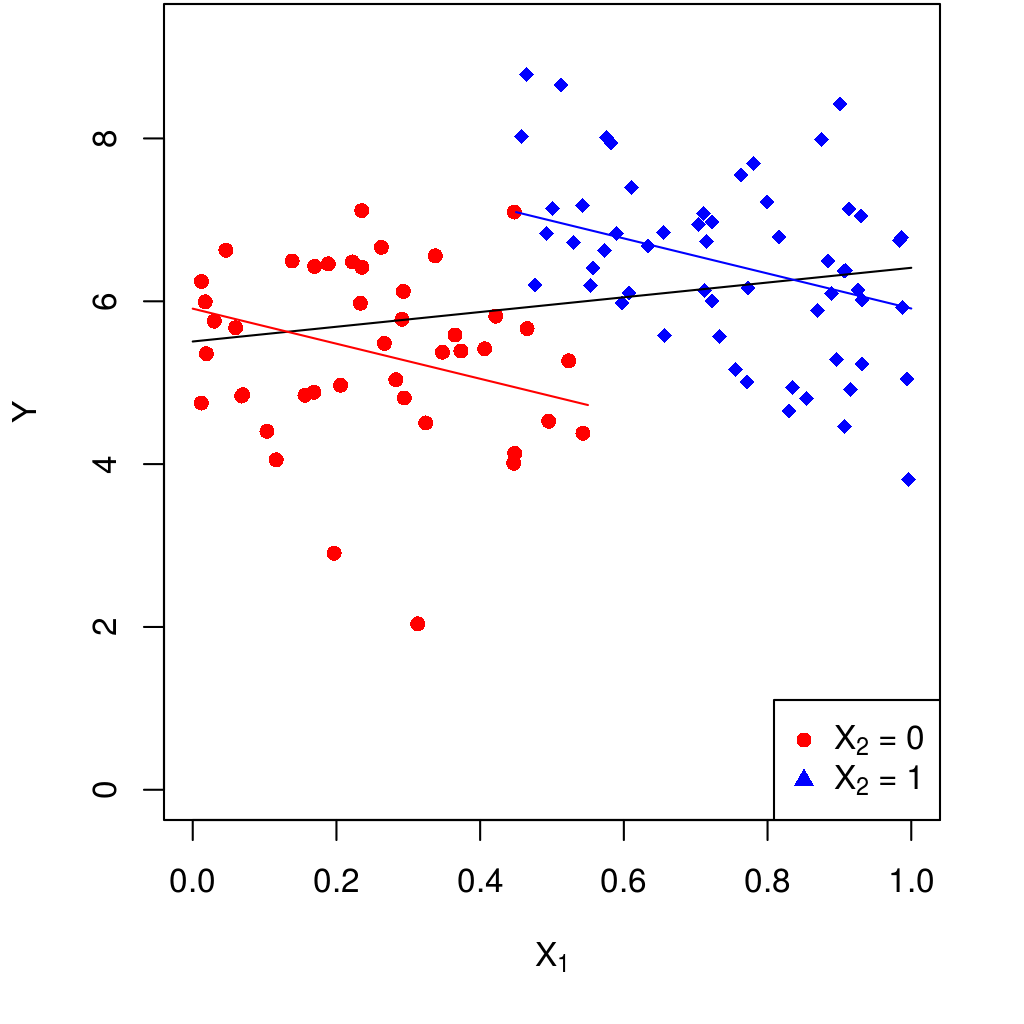
\includegraphics[width = 0.7\textwidth]{plots/confounding_colored_with_lines.png}
\end{frame}

\begin{frame}
\frametitle{Multiple regression: notation}
\end{frame}

\begin{frame}
\frametitle{Multiple regression: FEV}
\end{frame}


\section{Wrapping up}
\begin{frame}
\frametitle{SECTION 3: WRAPPING UP}
\end{frame}

\end{document}
